\section[Détermination empirique]{Détermination empirique}

\begin{frame}{Détermination empirique}
	\begin{itemize}
		\item Les régressions linéaire et logistique sont des algorithmes simples mais avec une théorie solide pour dériver des intervalles de confiances et des régions de prédictions à partir d'\textbf{un seul apprentissage}.
		\pause
		\item Ce n'est malheureusement pas le cas de tous les algorithmes d'apprentissage que l'on étudiera dans ce cours.
		\pause
		\item Dans cette section on verra comment on peut obtenir ces intervalles et régions de manière \textbf{empirique} et on comparera les résultats empiriques et théoriques obtenus précédemment.
		\item On utilisera l'algorithme du \textbf{bootstrapping} pour générer de \textbf{multiples} apprentissages et ainsi dériver ces intervalles et régions.
	\end{itemize}
\end{frame}

\begin{frame}{Notations pour les algorithmes}
	\begin{itemize}
		\item On note les $n$ observations des données d'apprentissage $\mathcal{D} = \{(x^{(i)}, y^{(i)})\}_{i=1}^n$.
		\item On note $\mathcal{D}^{(b)} \text{  pour  } b=1, 2, \cdots B$ les $B$ bootstraps générés.
		\item On note ${X_i^{(1)}, X_i^{(2)}, \cdots, X_i^{(m)}}$ les $m$ caractéristiques d'entrée pour l'inférence.
		\item On note $a: \mathcal{M}_{n,1}(\mathbb{R}) \to \mathbb{R}$ une fonction qui retourne un élément aléatoire d'un vecteur colonne $A$ en suivant une loi uniforme: $a(A) = A_j, \, j \sim \mathcal{U}(1, 2, \cdots, n)$.
	\end{itemize}
\end{frame}

\begin{frame}[allowframebreaks]{Régression linéaire}
	\begin{enumerate}
		\item Calculer $\hat{\beta}$ en utilisant toutes les données d'apprentissage $\mathcal{D}$ avec la méthode des moindres carrés.
		\item Calculer les résidus sur $\mathcal{D}$: $R = Y - \hat{Y}$.
		\item Répéter les étapes suivantes pour chaque bootstrap $b$:
		\begin{itemize}
			\item Déterminer les données d'apprentissage $\mathcal{D}^{(b)}$.
			\item Calculer $\hat{\beta}^{(b)}$ par la méthode des moindres carrés sur $\mathcal{D}^{(b)}$.
			\item Calculer $\hat{Y}_i^{(b)}$ à partir des données d'inférence $X_i$: $\hat{Y}_i^{(b)} = \Phi(X_i) \hat{\beta}^{(b)}$.
		\end{itemize}
		\item Pour chaque entrée $k$ de $X_i$, calculer les quantiles $\alpha / 2$ et $1 - \alpha / 2$ sur $\{\left(\hat{y}_i^{(k)}\right)^{(1)}, \left(\hat{y}_i^{(k)}\right)^{(2)}, \cdots, \left(\hat{y}_i^{(k)}\right)^{(B)}\}$. Cela donne l'intervalle de confiance au niveau $1 - \alpha$ pour $X_i^{(k)}$.
		\item Pour chaque bootstrap $b$ et tous les $X_i$, associer aléatoirement un résidu aux prédictions: $\left(\hat{y}_i^*\right)^{(b)} = \left(\hat{y}_i\right)^{(b)} + a(R)$.
		\item Pour chaque entrée $k$ de $X_i$, calculer les quantiles $\alpha / 2$ et $1 - \alpha / 2$ sur $\{\left(\hat{y}_i^{*(k)}\right)^{(1)}, \left(\hat{y}_i^{*(k)}\right)^{(2)}, \cdots, \left(\hat{y}_i^{*(k)}\right)^{(B)}\}$. Cela donne l'intervalle de prédiction au niveau $1 - \alpha$ pour $X_i^{(k)}$.
	\end{enumerate}
\end{frame}

\begin{frame}{Exemple: régression linéaire}
	\begin{columns}
		\begin{column}{0.5\textwidth}
			\begin{figure}
				\centering
				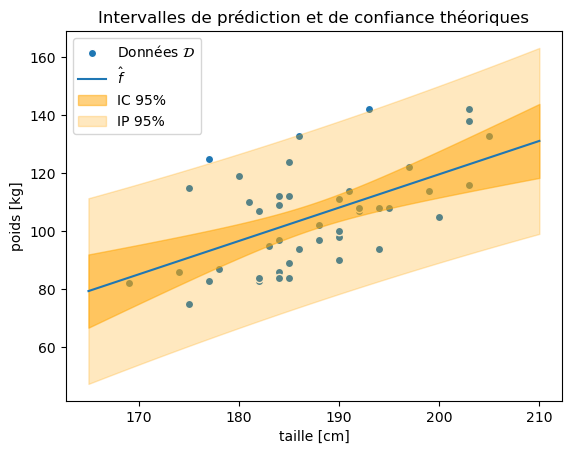
\includegraphics[width=1.0\linewidth]{Images/IP_IC_lineaire_theorie}
				\label{fig:IP_IC_lineaire_theorie}
			\end{figure}
		\end{column}
		\begin{column}{0.5\textwidth}
			\begin{figure}
				\centering
				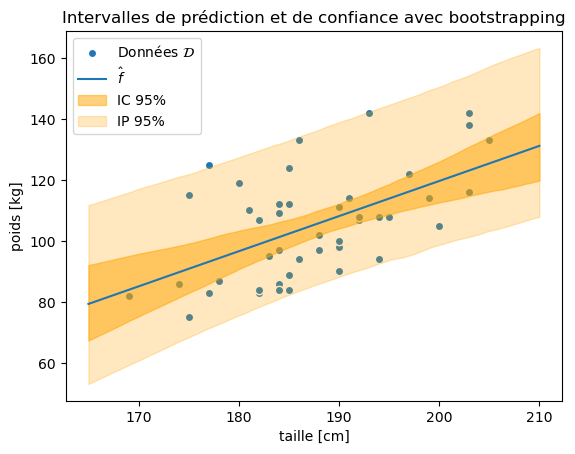
\includegraphics[width=1.0\linewidth]{Images/IP_IC_lineaire_bootstrap}
				\label{fig:IP_IC_lineaire_bootstrap}
			\end{figure}
		\end{column}
	\end{columns}
	Nous obtenons des résultats très similaires avec la théorie et avec un bootstrapping.
\end{frame}

\begin{frame}[allowframebreaks]{Régression logistique}
	\begin{enumerate}
		\item Calculer $\hat{\beta}$ en utilisant toutes les données d'apprentissage $\mathcal{D}$ avec la méthode des moindres carrés.
		\item Répéter les étapes suivantes pour chaque bootstrap $b$:
		\begin{itemize}
			\item Déterminer les données d'apprentissage $\mathcal{D}^{(b)}$.
			\item Calculer $\hat{\beta}^{(b)}$ sur $\mathcal{D}^{(b)}$ avec une régression logistique.
			\item Calculer $\hat{p}_i^{(b)}$ à partir des données d'inférence $X_i$: $\hat{p}_i^{(b)} = \sigma\left(\Phi(X_i) \hat{\beta}^{(b)}\right)$.
		\end{itemize}
		\item Pour chaque entrée $k$ de $X_i$, calculer les quantiles $\alpha / 2$ et $1 - (\alpha / 2)$ sur $\{\left(\hat{p}_i^{(k)}\right)^{(1)}, \left(\hat{p}_i^{(k)}\right)^{(2)}, \cdots, \left(\hat{p}_i^{(k)}\right)^{(B)}\}$. Cela donne l'intervalle de confiance au niveau $1 - \alpha$ pour $X_i^{(k)}$.
		\item Pour chaque entrée $k$ de $X_i$, on détermine l'espace de prédiction $C\left(x_i^{(k)}\right)$ d'une manière similaire à l'approche théorique:
		\begin{equation}
			C\left(x_i^{(k)}\right) = 
			\begin{cases}
				\{0\} & \text{si} \, \hat{p}_{1-\alpha/2}^{(k)} \le \alpha \\
				\{1\} & \text{si} \, \hat{p}_{\alpha/2}^{(k)} \ge 1 - \alpha \\
				\{0, 1\} & \text{sinon}
			\end{cases}
			\nonumber
		\end{equation}		
	\end{enumerate}
\end{frame}

\begin{frame}{Exemple: régression logistique}
	\begin{columns}
		\begin{column}{0.5\textwidth}
			\begin{figure}
				\centering
				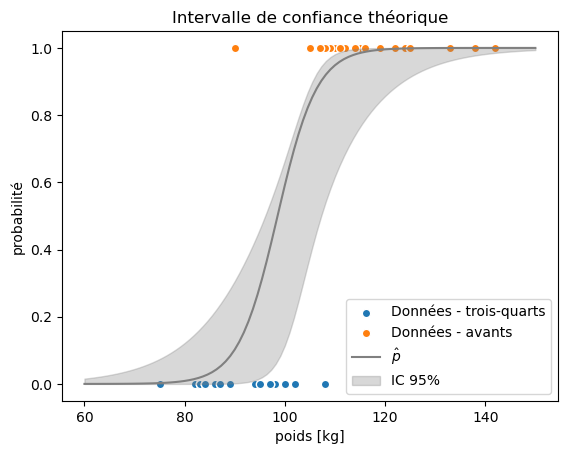
\includegraphics[width=1.0\linewidth]{Images/IP_IC_logistique_theorie}
				\label{fig:IP_IC_logistique_theorie}
			\end{figure}
		\end{column}
		\begin{column}{0.5\textwidth}
			\begin{figure}
				\centering
				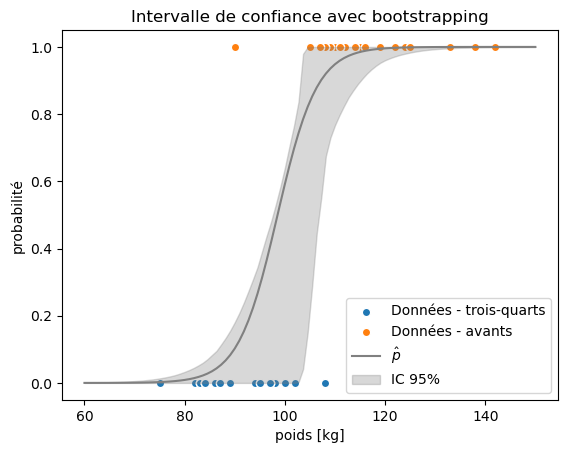
\includegraphics[width=1.0\linewidth]{Images/IP_IC_logistique_bootstrap}
				\label{fig:IP_IC_logistique_bootstrap}
			\end{figure}
		\end{column}
	\end{columns}
	Nous obtenons des résultats assez similaires avec la théorie et avec un bootstrapping.
\end{frame}

\begin{frame}{Exemple: régression logistique}
	\begin{columns}
		\begin{column}{0.5\textwidth}
			\begin{figure}
				\centering
				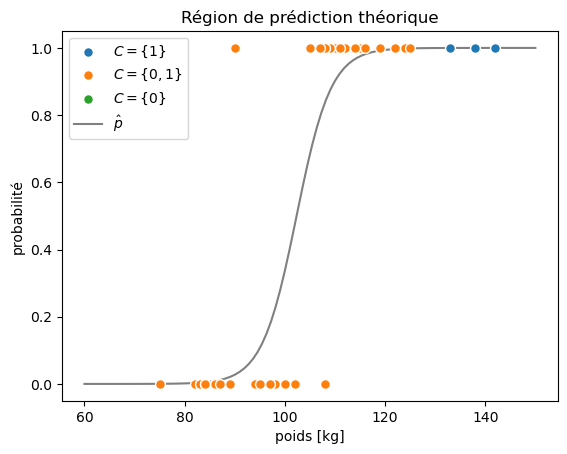
\includegraphics[width=0.95\linewidth]{Images/region_prediction_theorique}
				\label{fig:region_prediction_theorique}
			\end{figure}
		\end{column}
		\begin{column}{0.5\textwidth}
			\begin{figure}
				\centering
				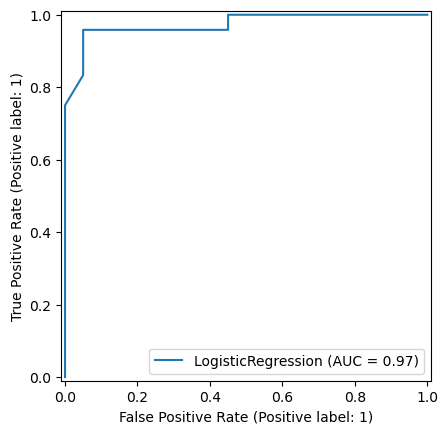
\includegraphics[width=0.85\linewidth]{Images/ROC}
				\label{fig:ROC}
			\end{figure}
		\end{column}
	\end{columns}
	Même si la courbe ROC montre que notre algorithme capture bien les tendances, la region de prédiction est beaucoup plus exigeante et ne montre que quelques (5) joueurs classés avec confiance comme des avants. Pour tous les autres joueurs, la régression logistique est beaucoup moins catégorique.
\end{frame}
